\documentclass{article}
\usepackage{amsmath}
\usepackage{graphicx}
\usepackage[table,xcdraw]{xcolor}
\usepackage{matlab-prettifier}
\usepackage{multicol}
 \usepackage[top=30mm, bottom=30mm, left=30mm, right=30mm,includehead=true,includefoot=true]{geometry}
\usepackage{calc}
\usepackage{eso-pic}
\usepackage{placeins}
\usepackage{listings}
\usepackage{subcaption}
\usepackage{subfigure}

%% for text superscript

\usepackage{fixltx2e}

%%%%%
%% for the medium size matrix
\usepackage{amsmath}
\usepackage{nccmath}
\newenvironment{mpmatrix}{\begin{medsize}\begin{pmatrix}}%
{\end{pmatrix}\end{medsize}}%
%%%%

\usepackage[bookmarks,hypertexnames=false,debug,linktocpage=true,hidelinks]{hyperref}
\hypersetup{
    colorlinks,
    linktoc=all,
    linkcolor={blue},
    citecolor={blue},
    urlcolor={blue}
}

%\settextfont[Scale = 1]{B Nazanin}
% \linespread{3}

% Border
\newlength{\PageFrameTopMargin}
\newlength{\PageFrameBottomMargin}
\newlength{\PageFrameLeftMargin}
\newlength{\PageFrameRightMargin}

\setlength{\PageFrameTopMargin}{1cm}
\setlength{\PageFrameBottomMargin}{1cm}
\setlength{\PageFrameLeftMargin}{1cm}
\setlength{\PageFrameRightMargin}{1cm}

\makeatletter

\newlength{\Page@FrameHeight}
\newlength{\Page@FrameWidth}

\AddToShipoutPicture{
  \thinlines
  \setlength{\Page@FrameHeight}{\paperheight-\PageFrameTopMargin-\PageFrameBottomMargin}
  \setlength{\Page@FrameWidth}{\paperwidth-\PageFrameLeftMargin-\PageFrameRightMargin}
  \put(\strip@pt\PageFrameLeftMargin,\strip@pt\PageFrameTopMargin){
    \framebox(\strip@pt\Page@FrameWidth, \strip@pt\Page@FrameHeight){}}}

\makeatother

% Border

\begin{document}

\begin{figure}
  \centering
  
\includegraphics[scale = 0.4]{images/kn-toosi.png}
\end{figure}


\title{MPC \\
       4\textsuperscript{th} Assignment}

\author{Reza Shahriari, 40308094}

\maketitle

\newpage

\section{Problem 1}
\subsection{Part A}
For designing the MPC Controller we first have to define the state space representation of the matrix in MATLAB. In the following code, the system is defined and discretized.

\begin{lstlisting}[frame=single,numbers=left,style=Matlab-Pyglike]
function [xplus,yd]= SystemDynamics(xd,ud)

% Parameter Definition
M_S = 2500;
M_U = 320;
k_S = 80000;
k_U = 500000;
c_s = 350;
c_U = 15020;

A = [0     1        0          0;
     0 -c_s/M_S -k_S/M_S c_s/M_S;
     0     1          0       -1;
     -k_U/M_U c_s/M_U (k_S+k_U)/M_U -(c_s+c_U)/M_U];


B = [0 ; 1/M_S ; 0 ;1/M_U];

C = [1 0 0 0; 0 1 0 0; 0 0 1 0];

Ad = [0.9241    0.0945   -0.0672    0.0013;
   -2.0392    0.8450   -0.6570    0.0178;
    0.8830    0.0843   -0.1675    0.0021;
    1.2927    0.1390   -1.8258   -0.0591];

Bd = [    0.1053;
    2.2534;
   -0.8123;
  -51.0695];

Cd = C;

xplus = Ad*xd + Bd*ud;
yd = Cd*xd;
\end{lstlisting}

Then the system is defined in a Matlab Function, in SIMULINK. The SIMULINK configuration is as follows:

\begin{figure}
    \centering
    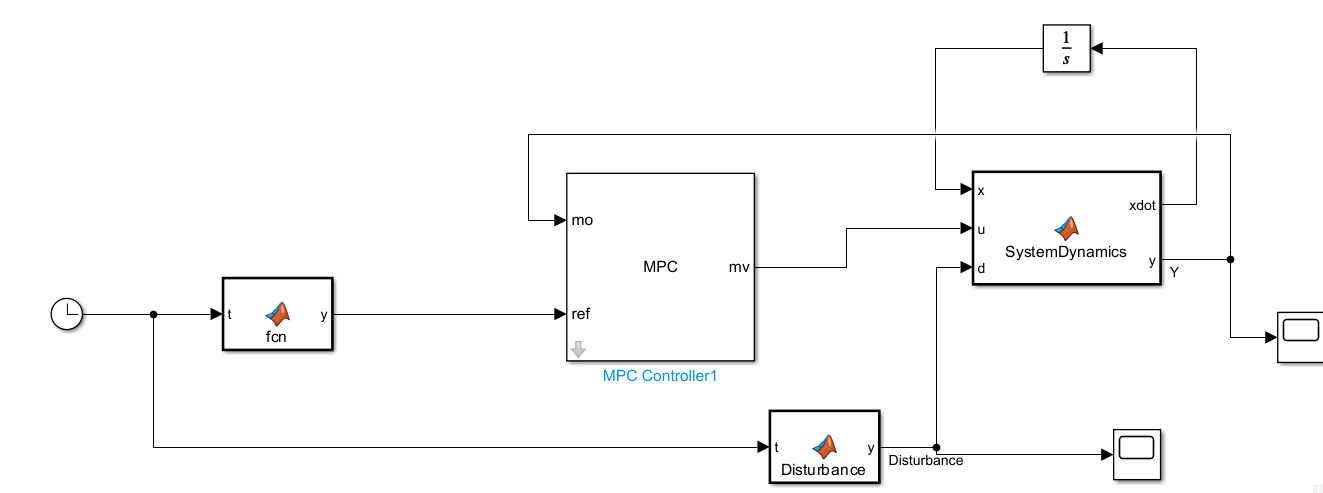
\includegraphics[width=\linewidth]{images/Linear_MPC_Configuration.png}
    \caption{The MPC Configuration}
    \label{fig:enter-label2}
\end{figure}

The disturbance is described as follows:

\begin{lstlisting}[frame=single, numbers=left, style=Matlab-Pyglike]
function y = Disturbance(t)

if t>=4 & t<5 
    y = t-4;
elseif t>=5 & t<7
    y = 1;
elseif t>=7 & t<8
    y = -t+8;
else 
    y = 0;
end

\end{lstlisting}

The Weights are defined as follows: 

\begin{figure}
    \centering
    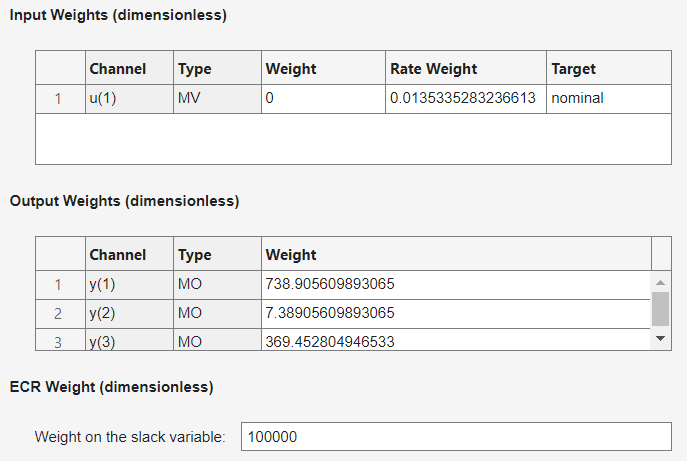
\includegraphics[width=0.5\linewidth]{images/Weights.png}
    \caption{Shows the weights}
    \label{fig:enter-label3}
\end{figure}

The following shows the results of Linear MPC utilized on the system.

\begin{figure}
    \centering
    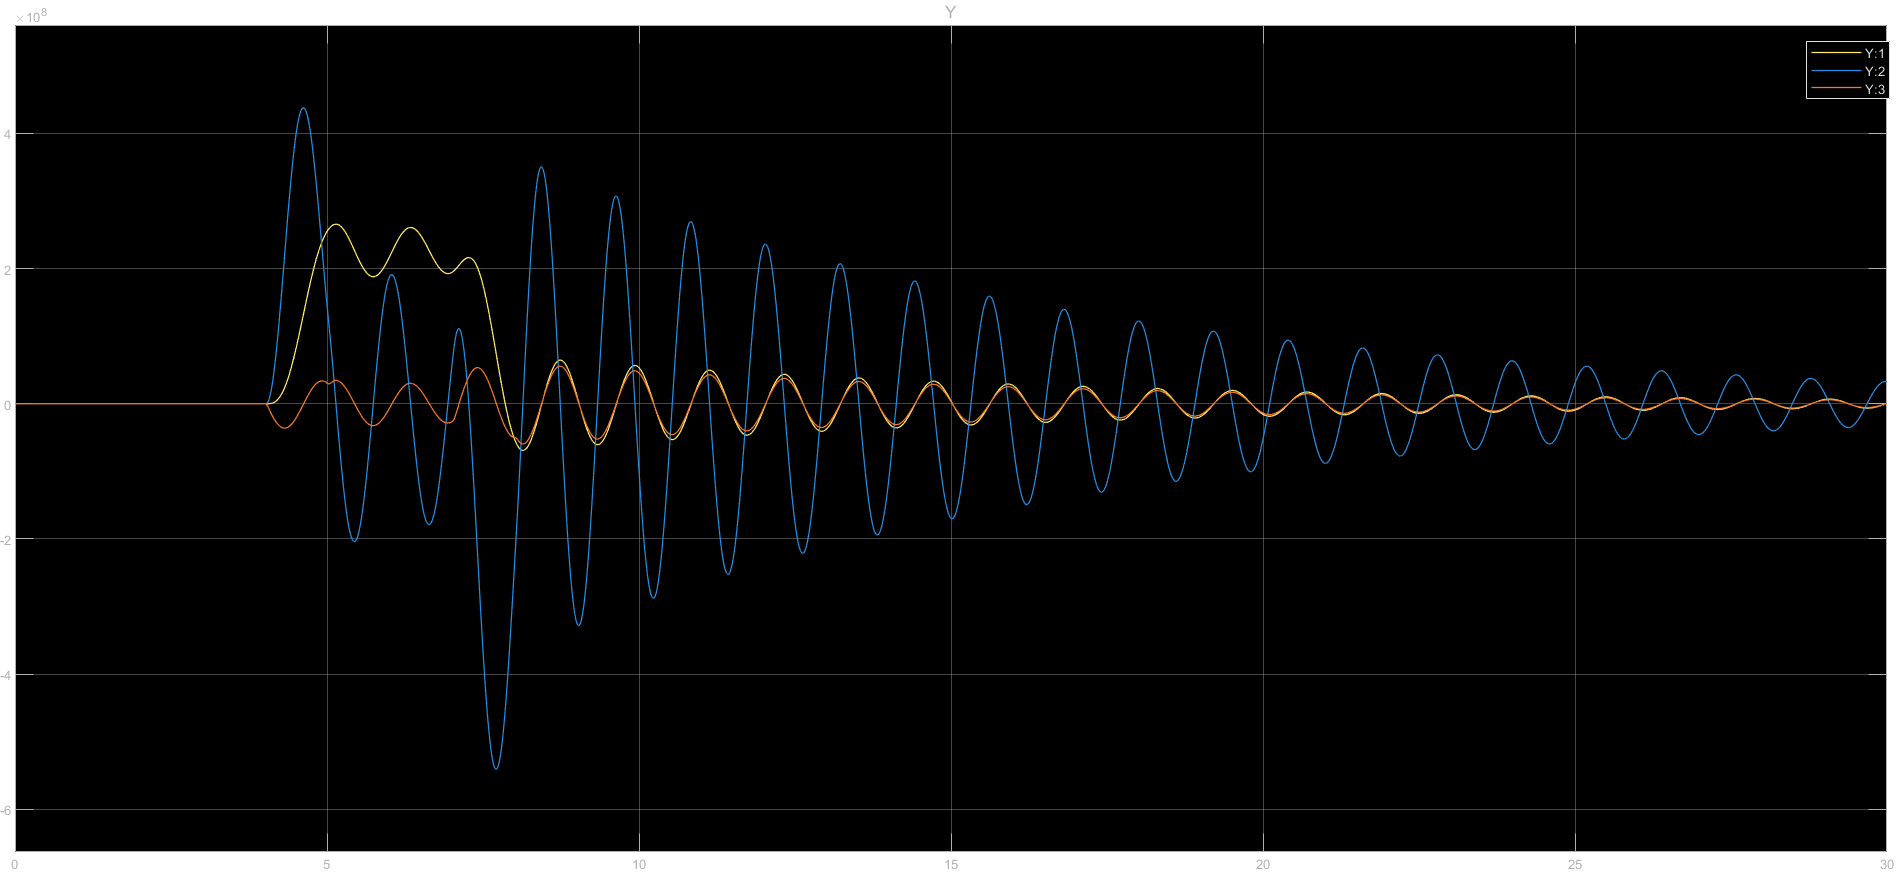
\includegraphics[width=\linewidth]{images/MPC_Results.png}
    \caption{Shows the results of MPC}
    \label{fig:enter-label4}
\end{figure}

The root mean square error of $x_1$ and $x_3$ can be calculated using following configuration.

\begin{figure}
    \centering
    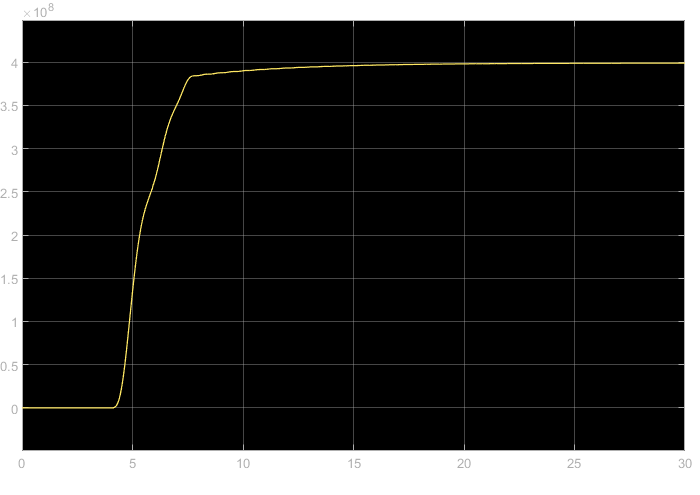
\includegraphics[width=\linewidth]{images/RMSE(Of X1).png}
    \caption{Root Mean Square Error of X1}
    \label{fig:enter-label5}
\end{figure}

\begin{figure}
    \centering
    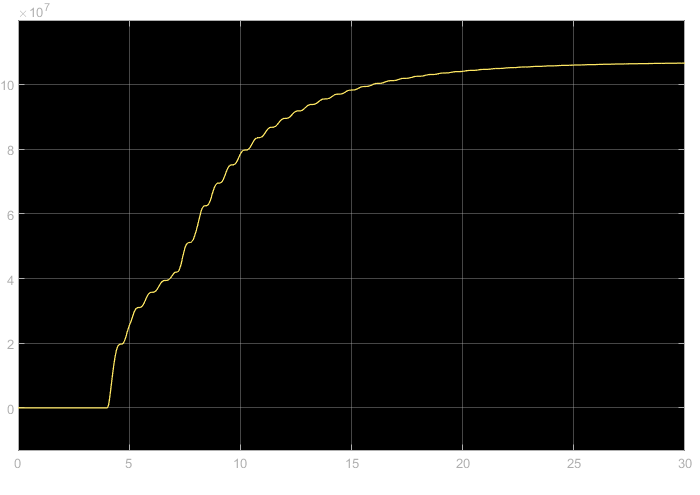
\includegraphics[width=\linewidth]{images/RMSE(Of X3).png}
    \caption{Root Mean Square Error of X2}
    \label{fig:enter-label6}
\end{figure}

\begin{figure}
    \centering
    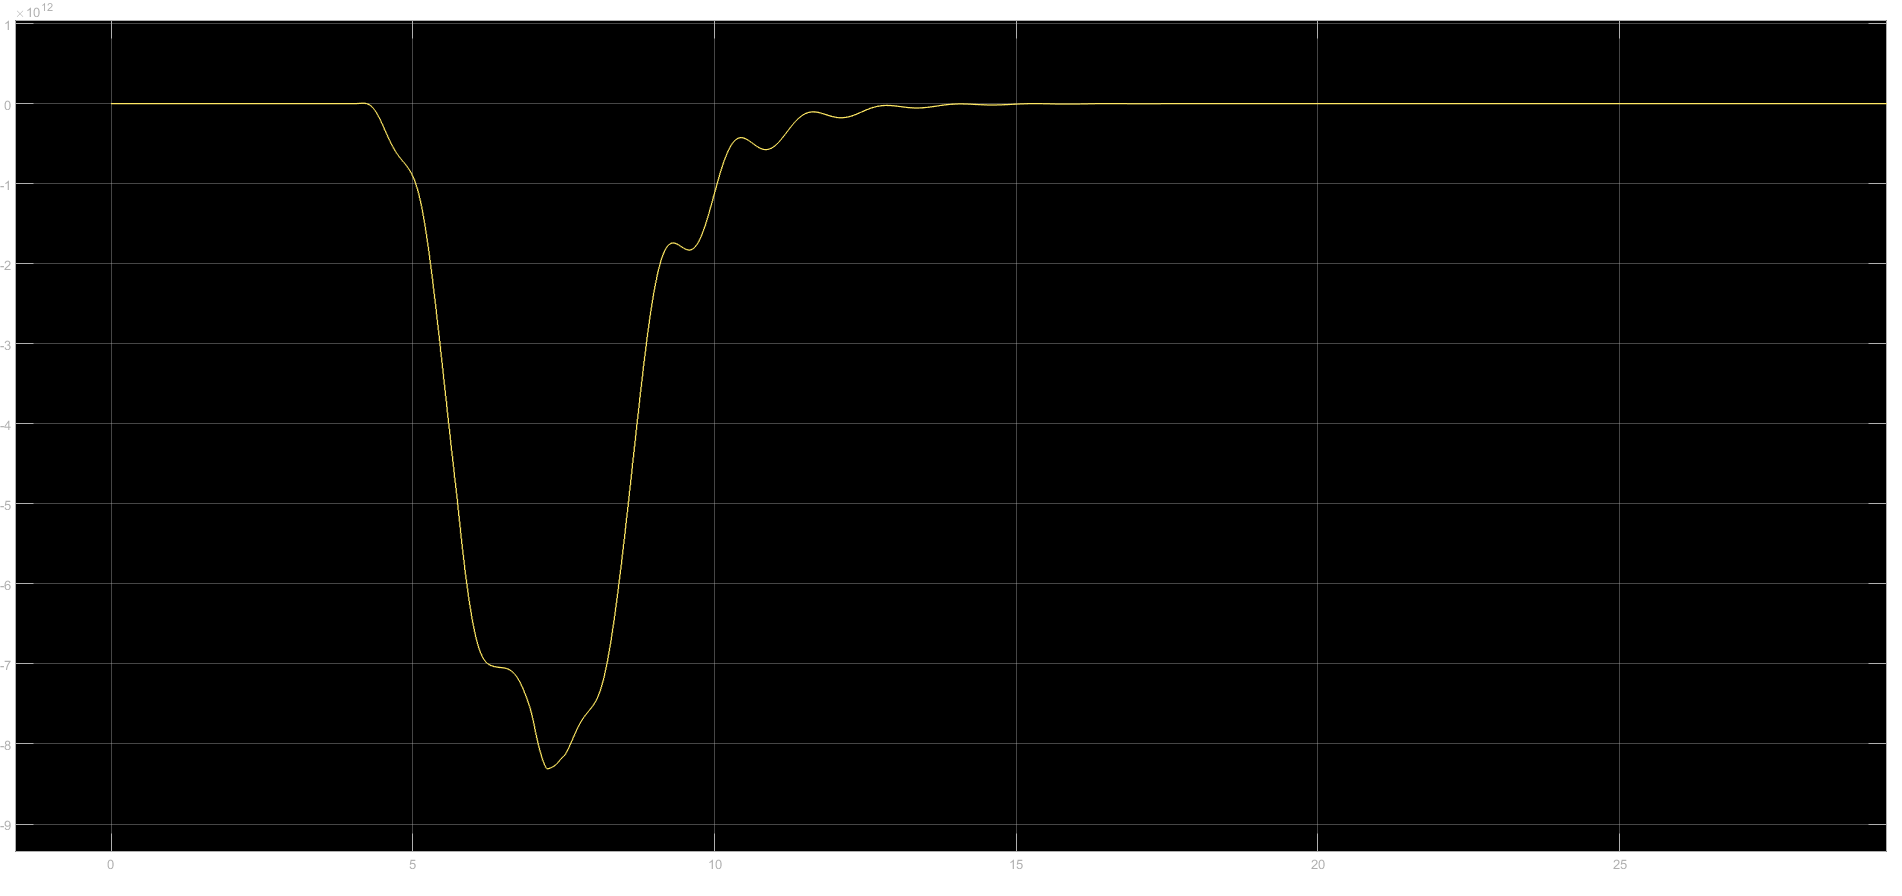
\includegraphics[width=\linewidth]{images/Control Effort.png}
    \caption{The Control Effort of the system}
    \label{fig:enter-label}
\end{figure}

The Output of PID controller is show in figure \ref{fig:enter-labe1} to compare with the results of MPC

The PID Parameters are as shown in figure \ref{fig3}:

\begin{figure}
    \centering
    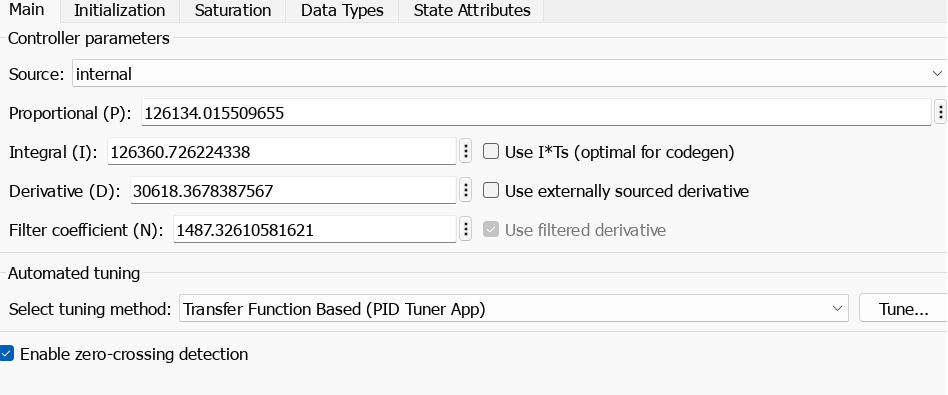
\includegraphics[width=\linewidth]{images/PID_Parameters.png}
    \caption{The PID Parameters}
    \label{fig3}
\end{figure}

\begin{figure}
    \centering
    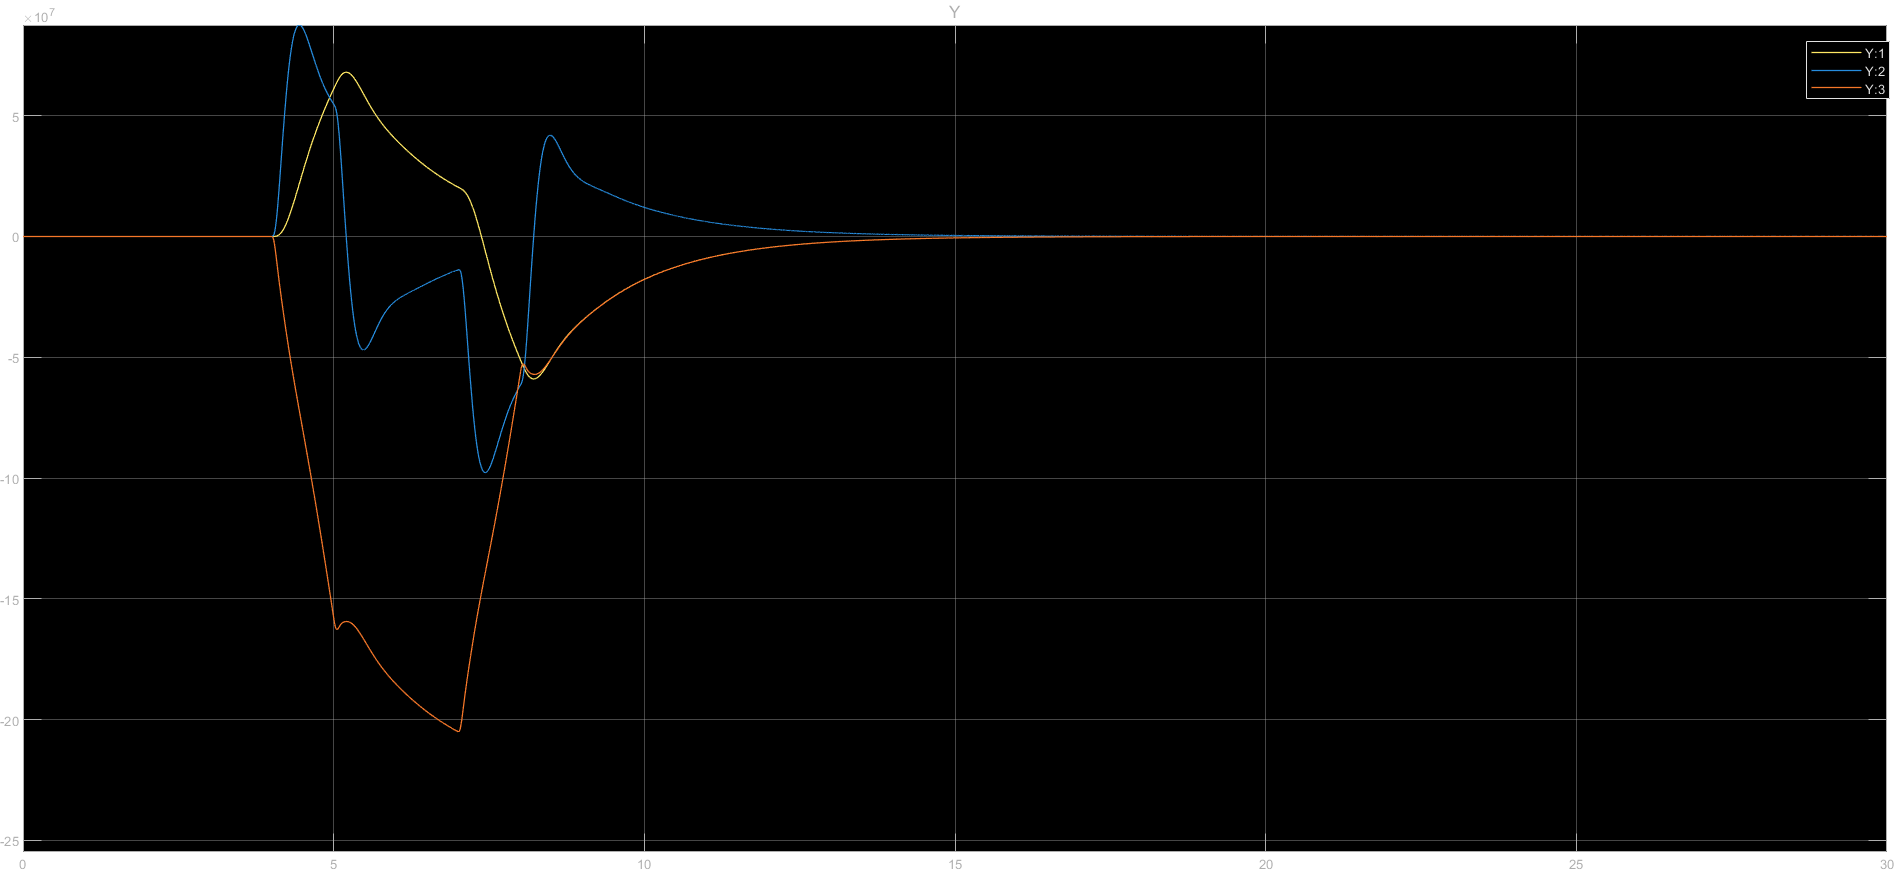
\includegraphics[width=\linewidth]{images/PID_Controller_Output.png}
    \caption{PID Controller output}
    \label{fig:enter-labe1}
\end{figure}

The Control effort of PID is shown in figure \ref{fig:enter-lab2} to compare with results of MPC

\begin{figure}
    \centering
    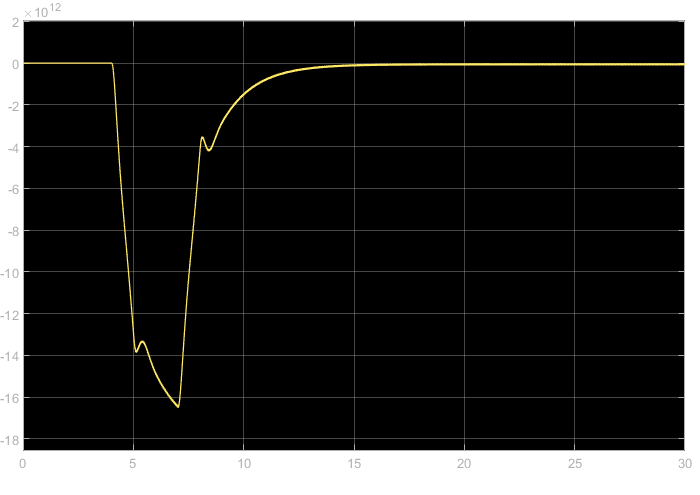
\includegraphics[width=\linewidth]{images/PID_Control_Effort.png}
    \caption{The Control Effort of PID}
    \label{fig:enter-lab2}
\end{figure}

The RMSE of X1 and X3 is given in figures \ref{fig1} and \ref{fig2} 

\begin{figure}
    \centering
    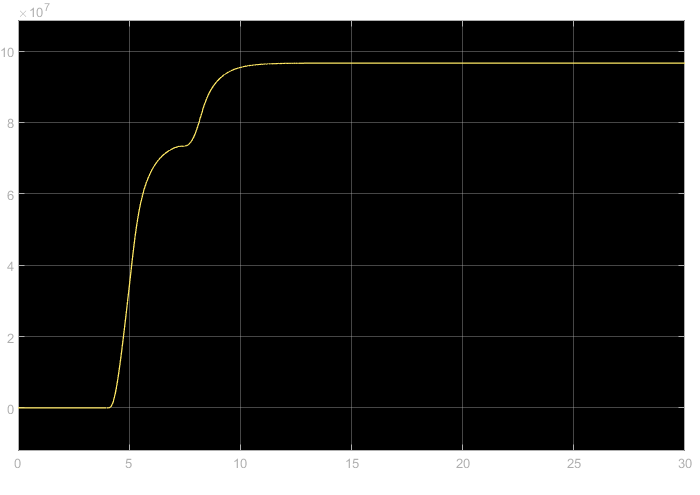
\includegraphics[width=\linewidth]{images/PID_RMSE_X1.png}
    \caption{RMSE of X1}
    \label{fig1}
\end{figure}

\begin{figure}
    \centering
    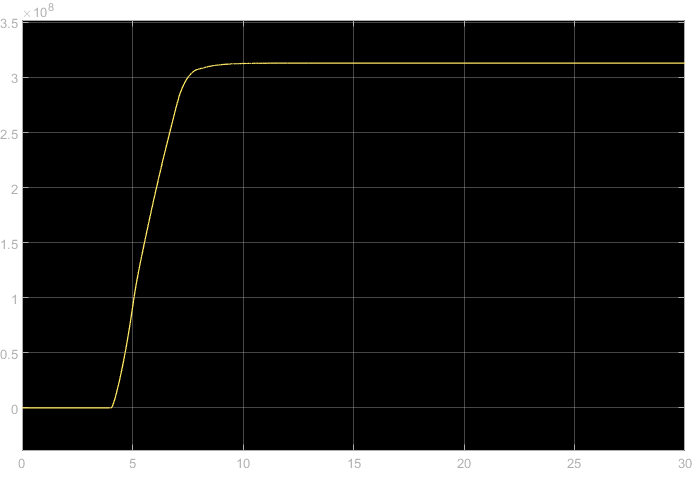
\includegraphics[width=\linewidth]{images/PID_RMSE_X2.png}
    \caption{RMSE of X3}
    \label{fig2}
\end{figure}

The control effort of PID shows a better signal than the Linear MPC and the output shows a better disturbance rejection, and shows a better RMSE in X1 and X3.

\subsection{Part B}
The tube MPC is simulated in this section, with adding a PID to the Linear MPC we previously had \ref{fig:Tube}, The Configuration bellow is utilized, It is worth noting that the previous linear MPC parameters are consistent with what we previously had, but the PID is tuned again the configuration in figure \ref{fig:PID_Tube} is presented as the new PID parameters.

\begin{figure}
    \centering
    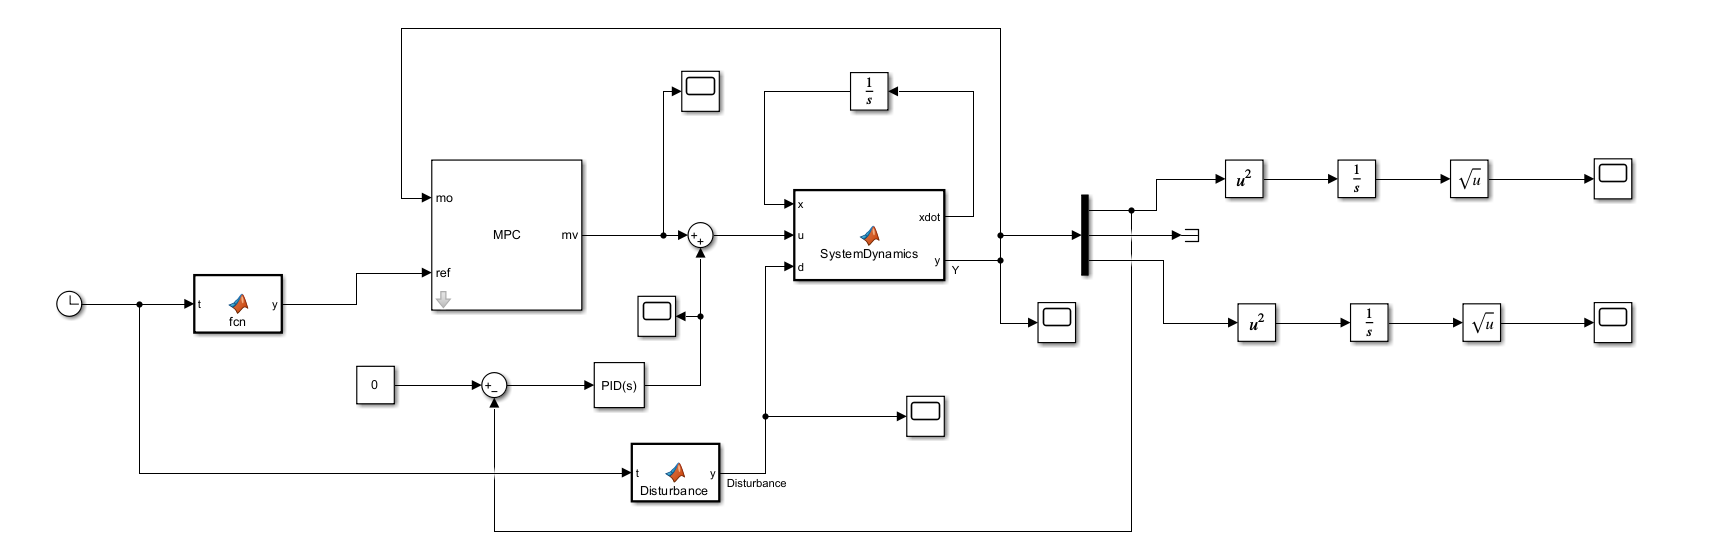
\includegraphics[width=\linewidth]{images/Tube_MPC_Configuration.png}
    \caption{The Configuration of Tube MPC}
    \label{fig:Tube}
\end{figure}

\begin{figure}
    \centering
    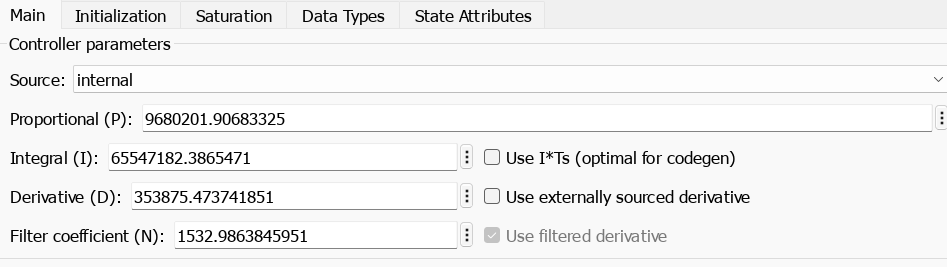
\includegraphics[width=\linewidth]{images/New_PID_Configuration.png}
    \caption{The new PID tuned}
    \label{fig:PID_Tube}
\end{figure}

The system output is given in \ref{fig:Tube:Result}. It shows magnificent disturbance rejection in the first and second output, but for the third output, not only was the disturbance not rejected, but it was amplified in the opposite direction. These results seem odd.

In figure \ref{fig:PID+MPC}, the control effort is shown.

\begin{figure}
    \centering
    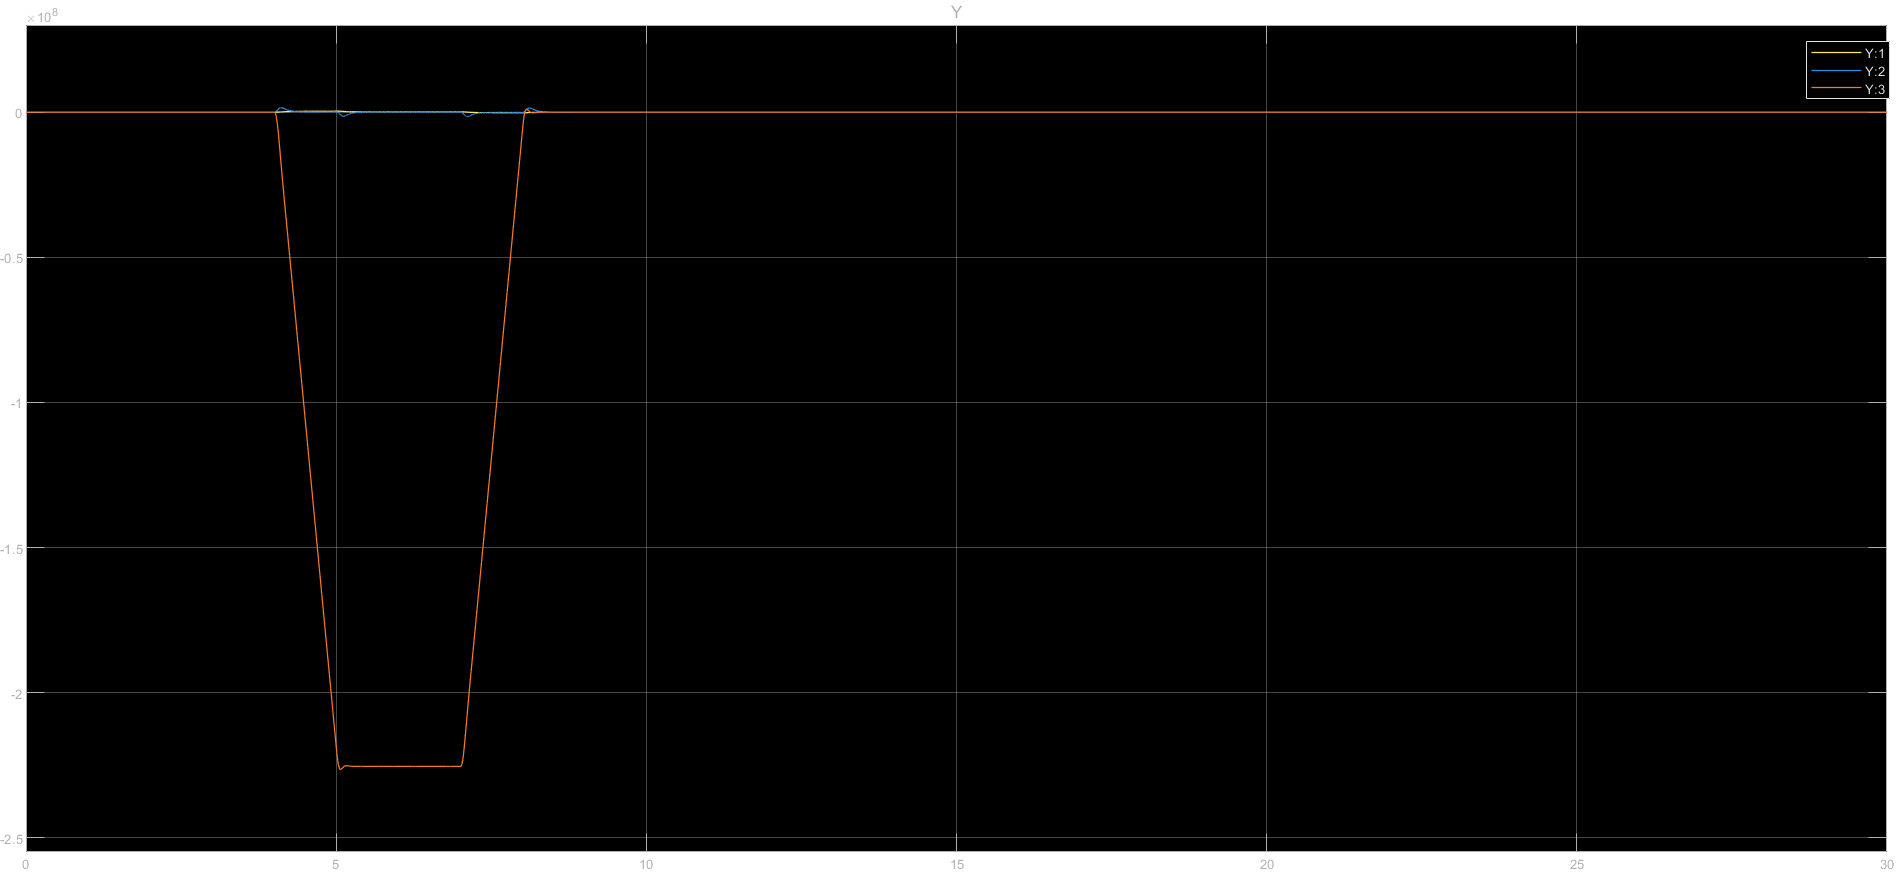
\includegraphics[width=\linewidth]{images/TUBE_MPC_RESULTS.png}
    \caption{The results of Tube MPC}
    \label{fig:Tube:Result}
\end{figure}

\begin{figure}
    \centering
    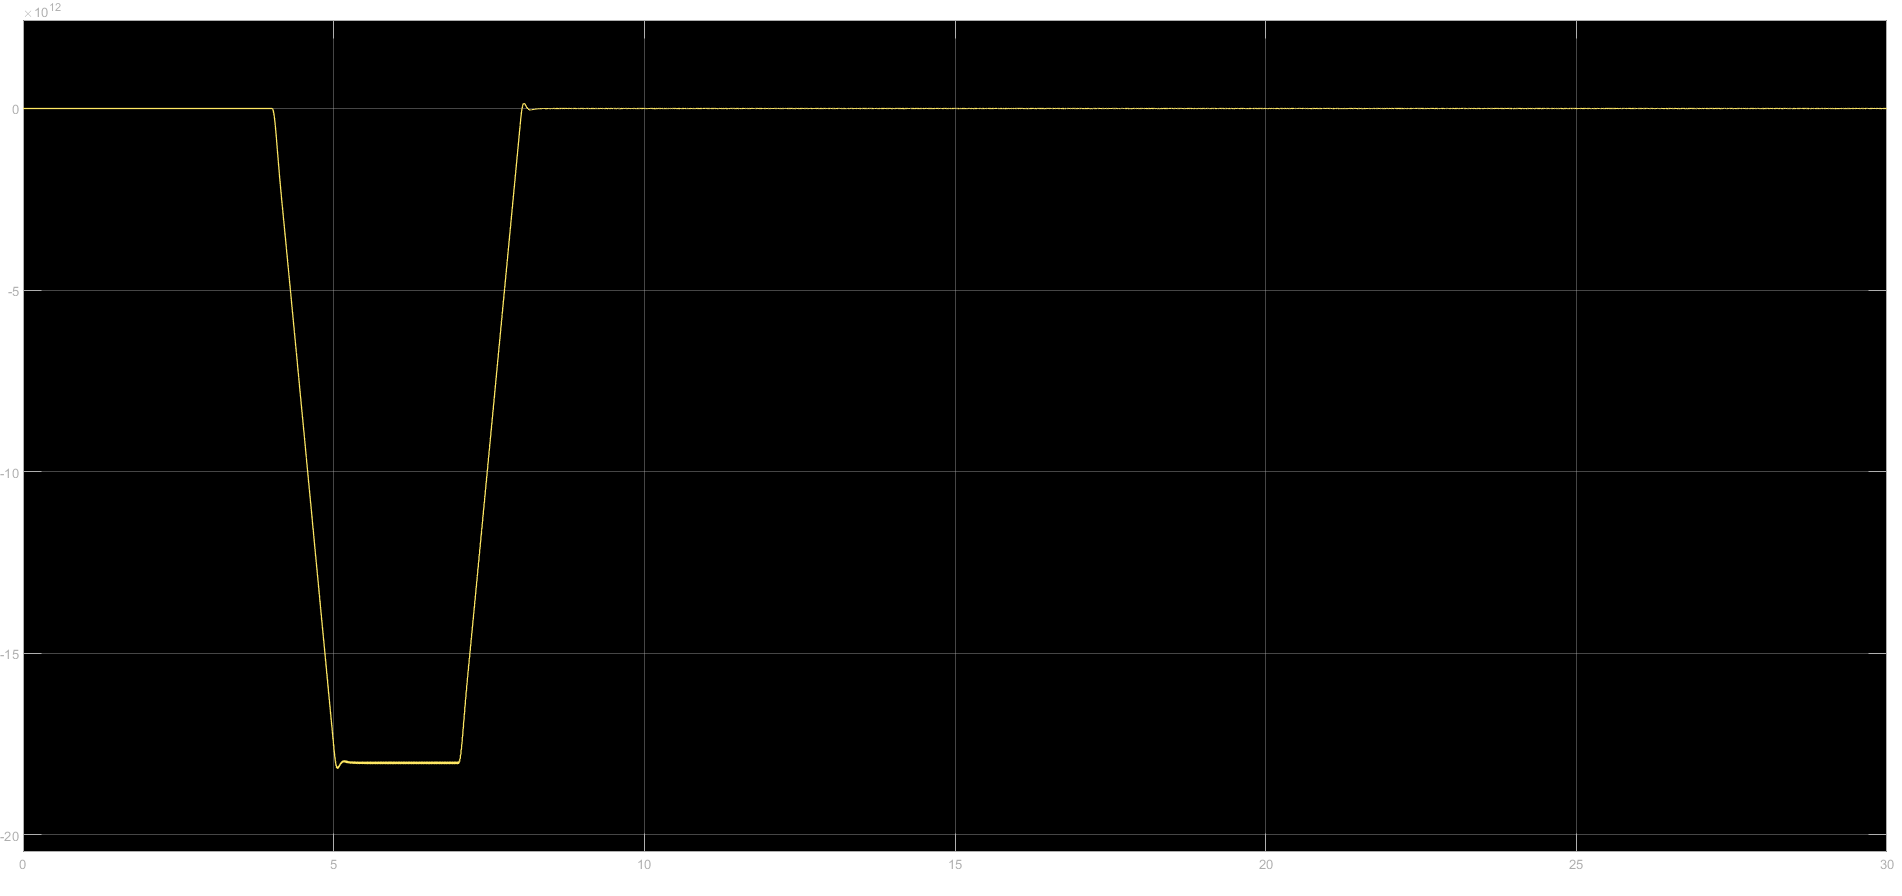
\includegraphics[width=\linewidth]{images/PID+MPC_Control_Output.png}
    \caption{PID+MPC Control Effort}
    \label{fig:PID+MPC}
\end{figure}

\FloatBarrier
\subsection{Part C}
For Tuning the explicit MPC, what we should first design the Linear MPC. This we have designed in Part A. Now in part C, to make the Linear MPC explicit we run the following two commands:

\begin{lstlisting}[frame=single,numbers=left,style=Matlab-Pyglike]
range = generateExplicitRange(mpc1)
explicit = generateExplicitMPC(mpc1,range)
\end{lstlisting}

This will create an explicit MPC object named "explicit". The range structure has seven states, in which the range of explicit making is defined. We have defined the min of each state to zero and its max to 1.

\begin{figure}[htbp]
    \centering
    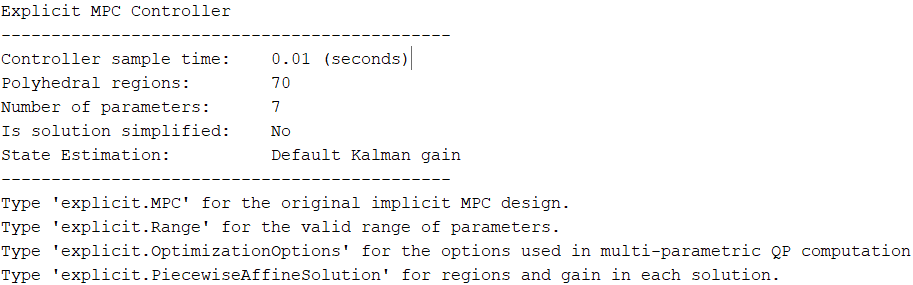
\includegraphics[width=\linewidth]{images/ExplicitMPC.png}
    \caption{The results of Explicit MPC}
    \label{fig:Exp}
\end{figure}

In figure \ref{fig:Exp} the results of the explicit MPC such as regions, type of filtering use, etc. are presented. The explicit MPC configuration follows like what we had with Linear MPC. The new configuration is shown in \ref{fig:ExplicitMPC}

\begin{figure}[htbp]
    \centering
    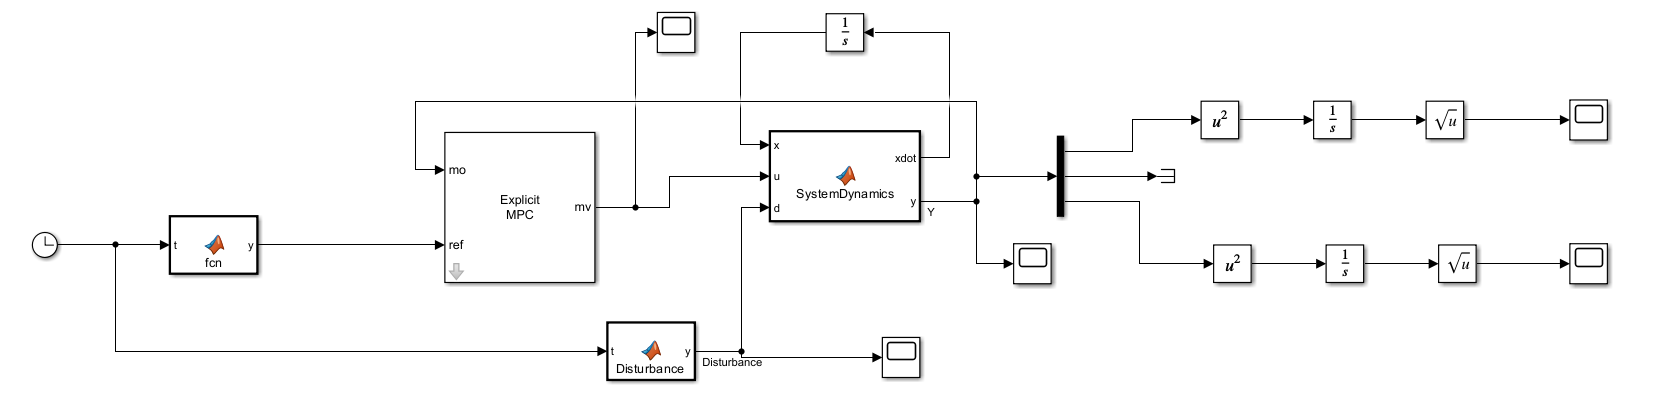
\includegraphics[width=\linewidth]{images/ExplicitConfig.png}
    \caption{The Configuration of Explicit MPC}
    \label{fig:ExplicitMPC}
\end{figure}

The result is also quite similar with what we had with Linear MPC in Part A. In figure \ref{fig:ExplictOutput}, the results of explicit MPC's output is presented, in \ref{fig:ControlEffort}, the control effort are shown. and figure \ref{fig:RMSE} a) shows the RMSE of X1 and b) shows the RMSE of X3 for when we have used the explicit MPC.

\begin{figure}[htbp]
    \centering
    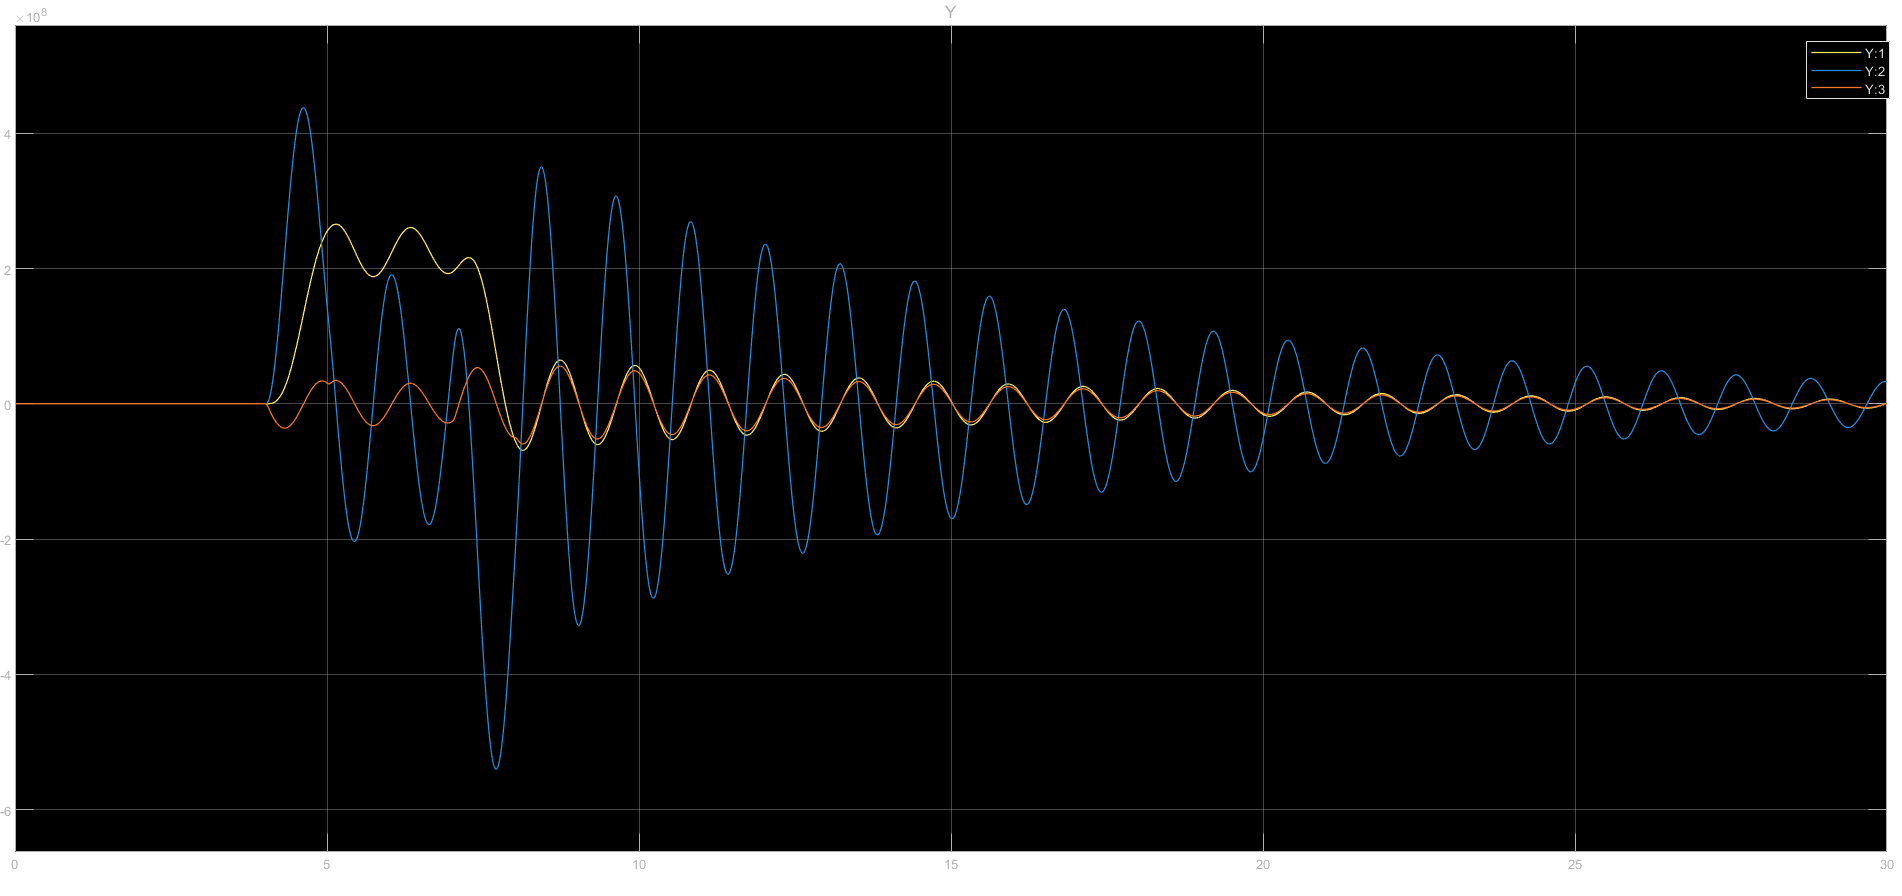
\includegraphics[width=\linewidth]{images/Explicit Output.png}
    \caption{The output of Explicit MPC}
    \label{fig:ExplictOutput}
\end{figure}

\begin{figure}[htbp]
    \centering
    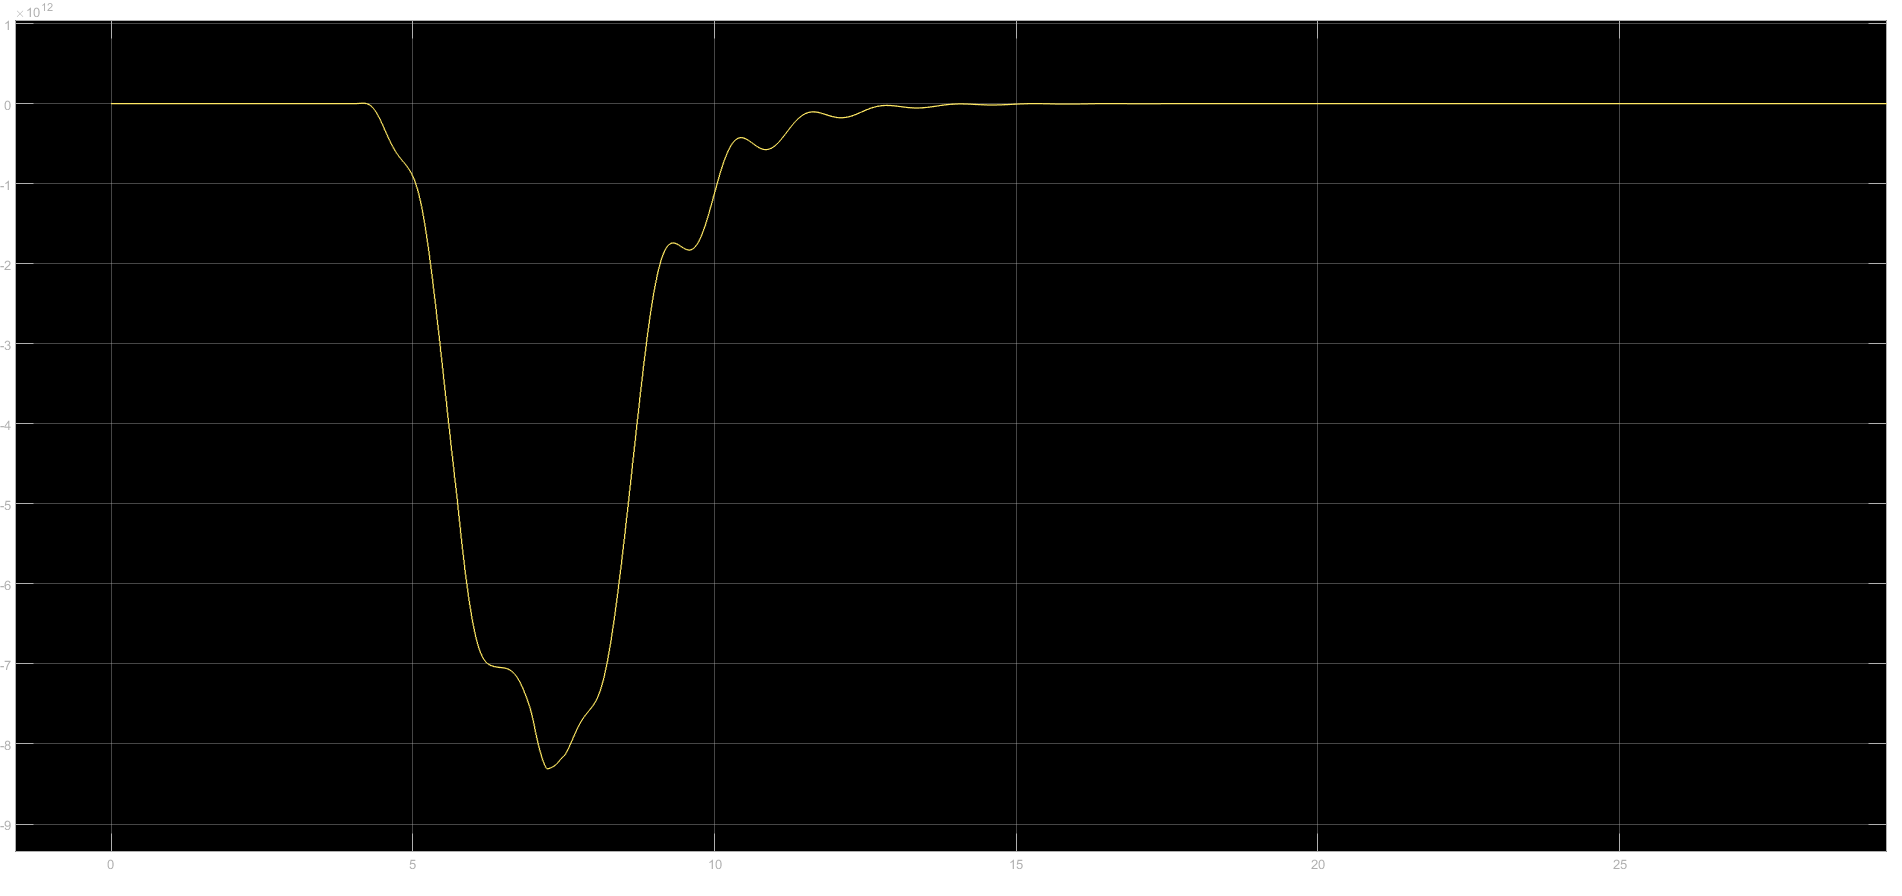
\includegraphics[width=\linewidth]{images/Control Effort.png}
    \caption{The control effort of Explicit MPC}
    \label{fig:ControlEffort}
\end{figure}

\begin{figure}[htbp]
    \centering
    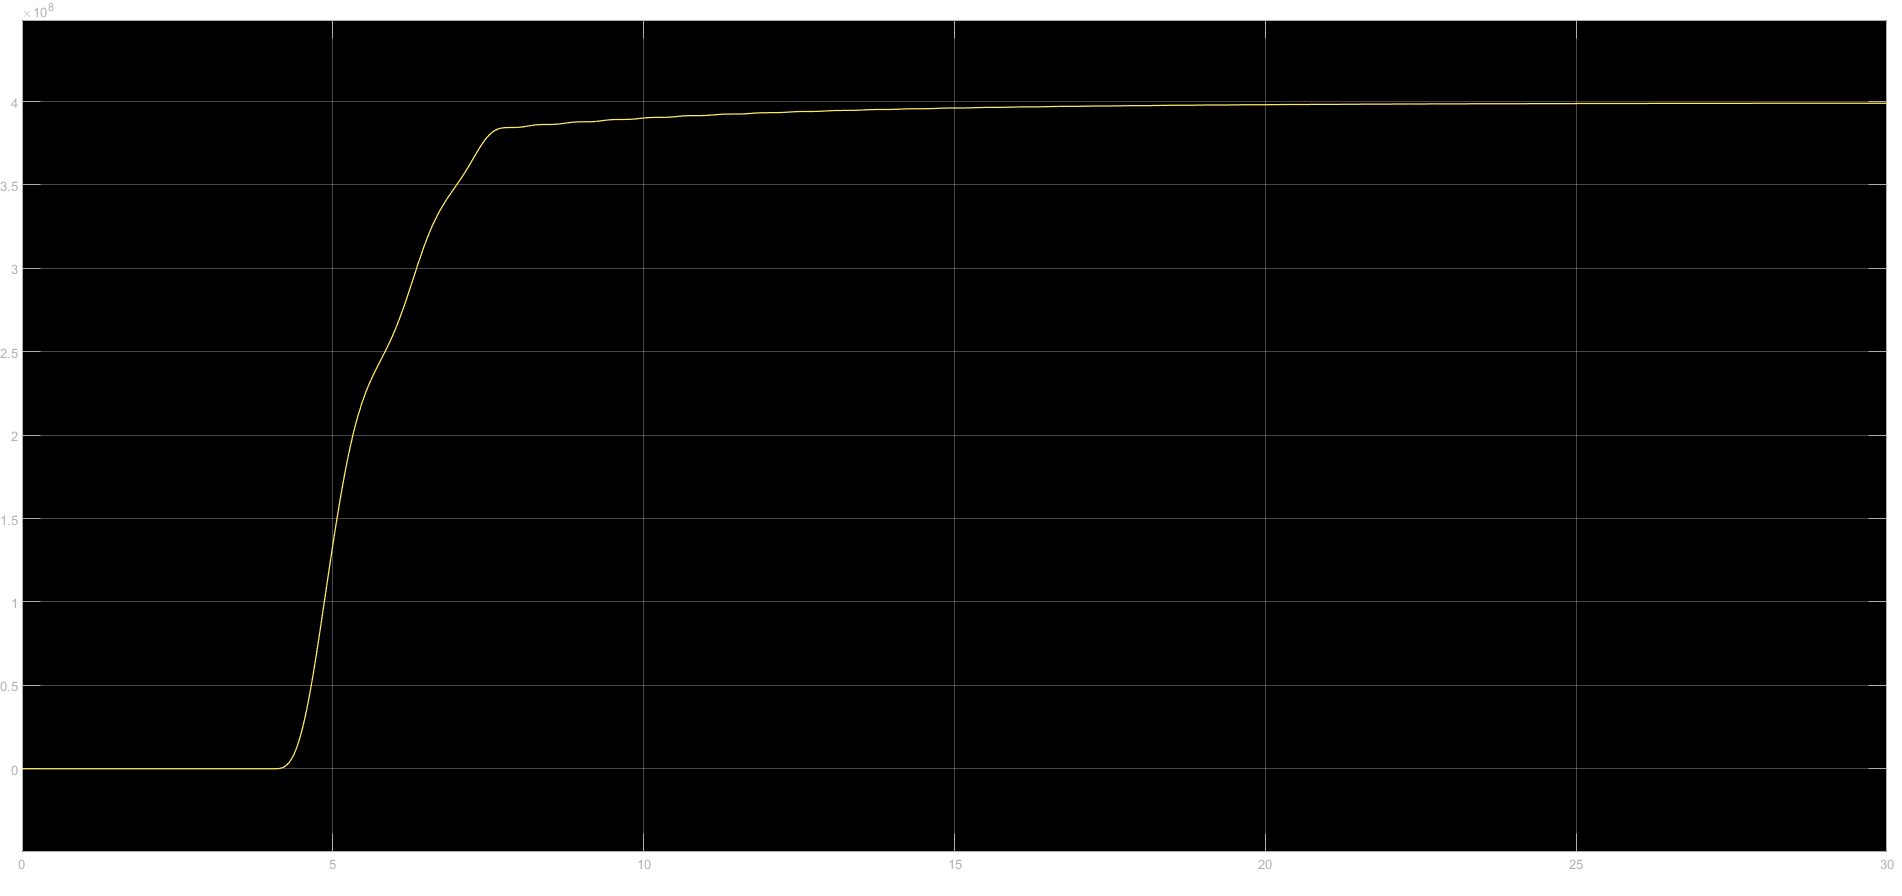
\includegraphics[width=0.5\linewidth]{images/ExplicitRMSE(X1).png}    
    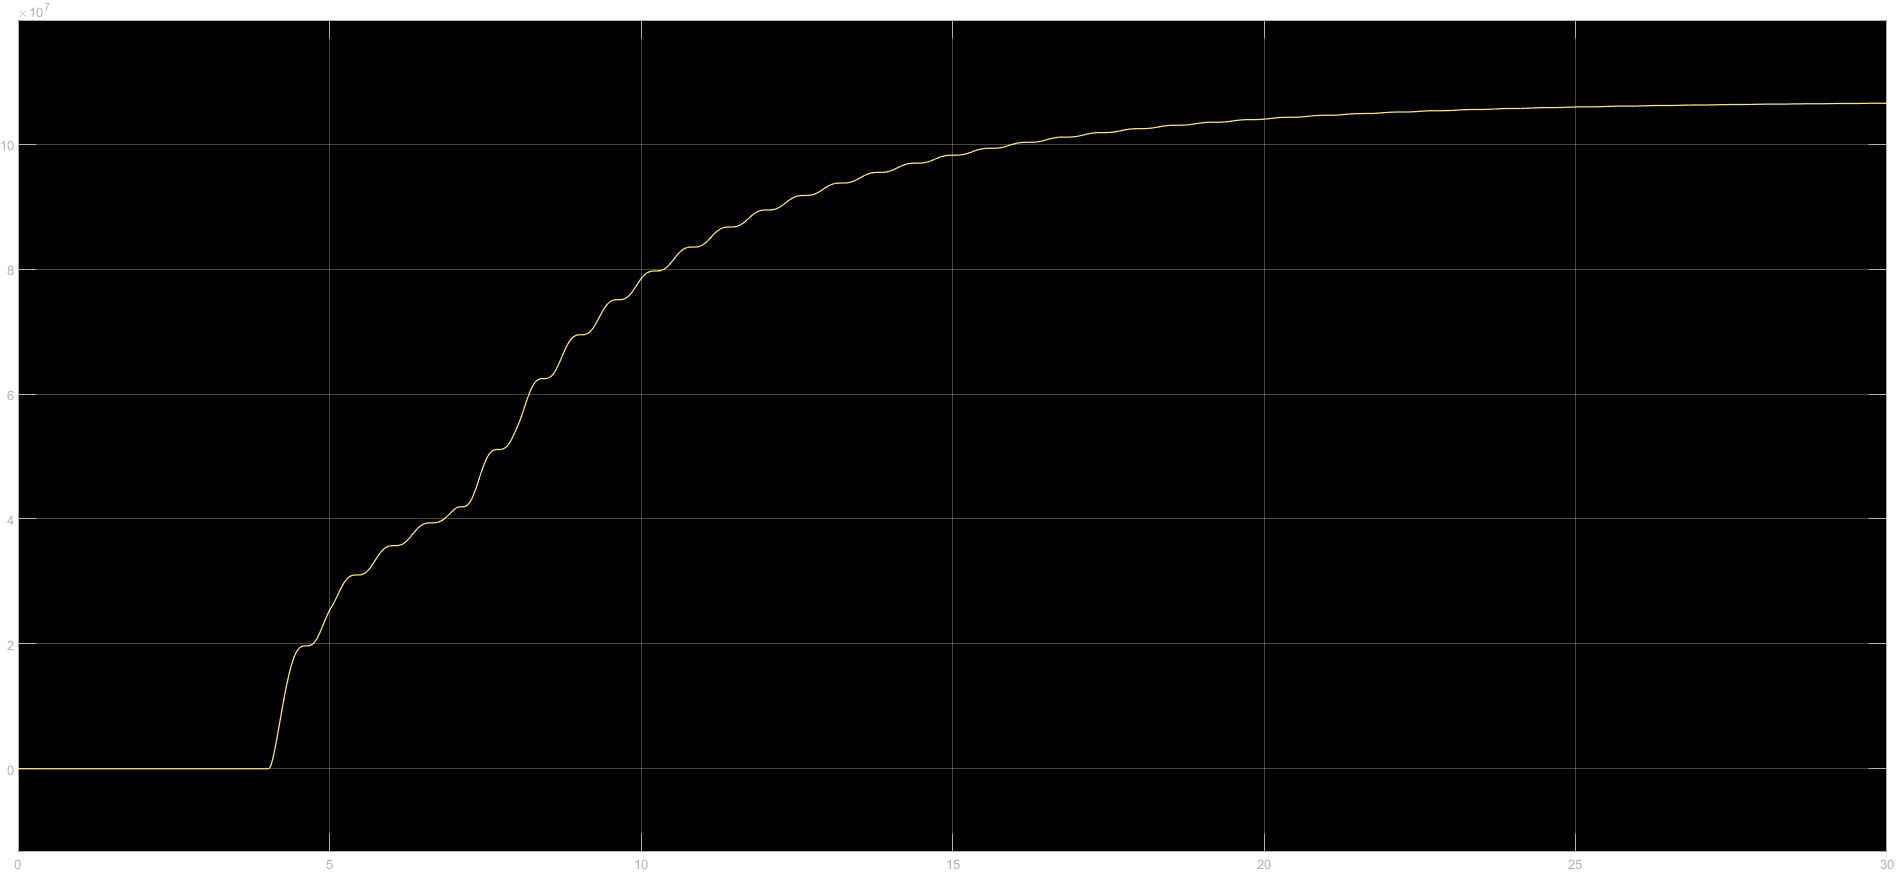
\includegraphics[width=0.5\linewidth]{images/ExplicitRMSE(X3).png}
    \caption{RMSE while implementing Explicit Control}
    \label{fig:RMSE}
\end{figure}

\FloatBarrier
\section{Problem 2}
In this problem a Hybrid MPC model is simulated. The baseline is a Linear MPC in reality. For the purose of this simulation we have made use of a switch that changes the dynamic used to create the output if a certain condition is satisfied. The general configuration is as follows in figure \ref{fig:HybridConfig}:

\begin{figure}[htbp]
    \centering
    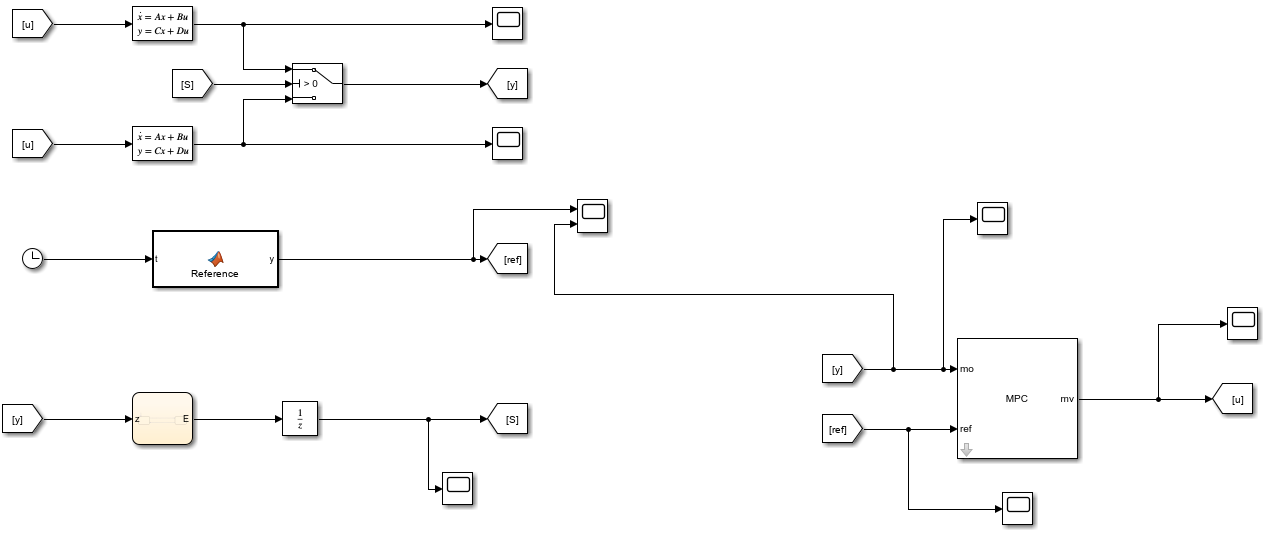
\includegraphics[width=\linewidth]{images/HybridMPC.png}
    \caption{The Hybrid MPC model}
    \label{fig:HybridConfig}
\end{figure}

The model was defined in the workspace using the following command lines:
\begin{lstlisting}[frame=single,numbers=left,style=Matlab-Pyglike]
A1 = [0 2 ; -2 -2];
B1 = [0;2];
A2 = [0 4; -4 -4]
B2 = [0;4]
C = [1 0]
\end{lstlisting}

Figure \ref{fig:weight} shows our state and input weights, and figure \ref{fig:Constraints} shows the input and output constraints.

\begin{figure}[htbp]
    \centering
    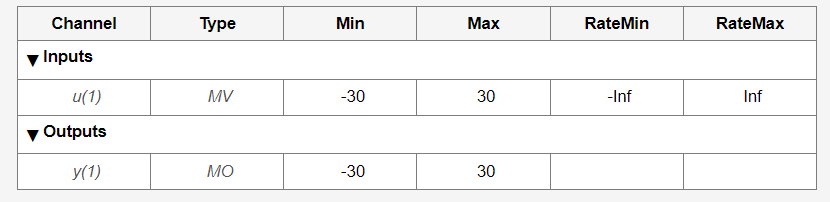
\includegraphics[width=\linewidth]{images/Constraints.png}
    \caption{Input and Output Constraints}
    \label{fig:Constraints}
\end{figure}

\begin{figure}[htbp]
    \centering
    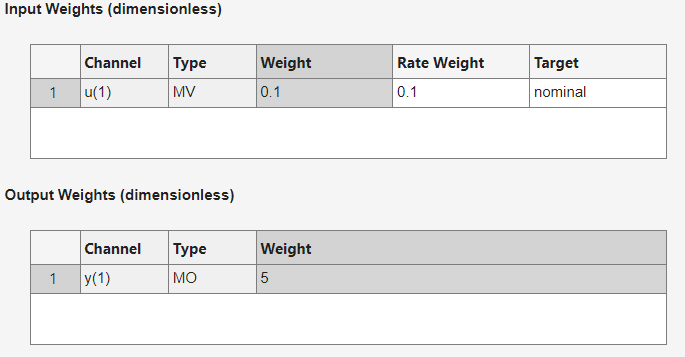
\includegraphics[width=\linewidth]{images/Input_Output_Weight.png}
    \caption{State and input weights}
    \label{fig:weight}
\end{figure}

The reference signal is defined as $20sin(\frac{2\pi}{20}t)$. Figure \ref{fig:reference} plots its reference

\begin{figure}[htbp]
    \centering
    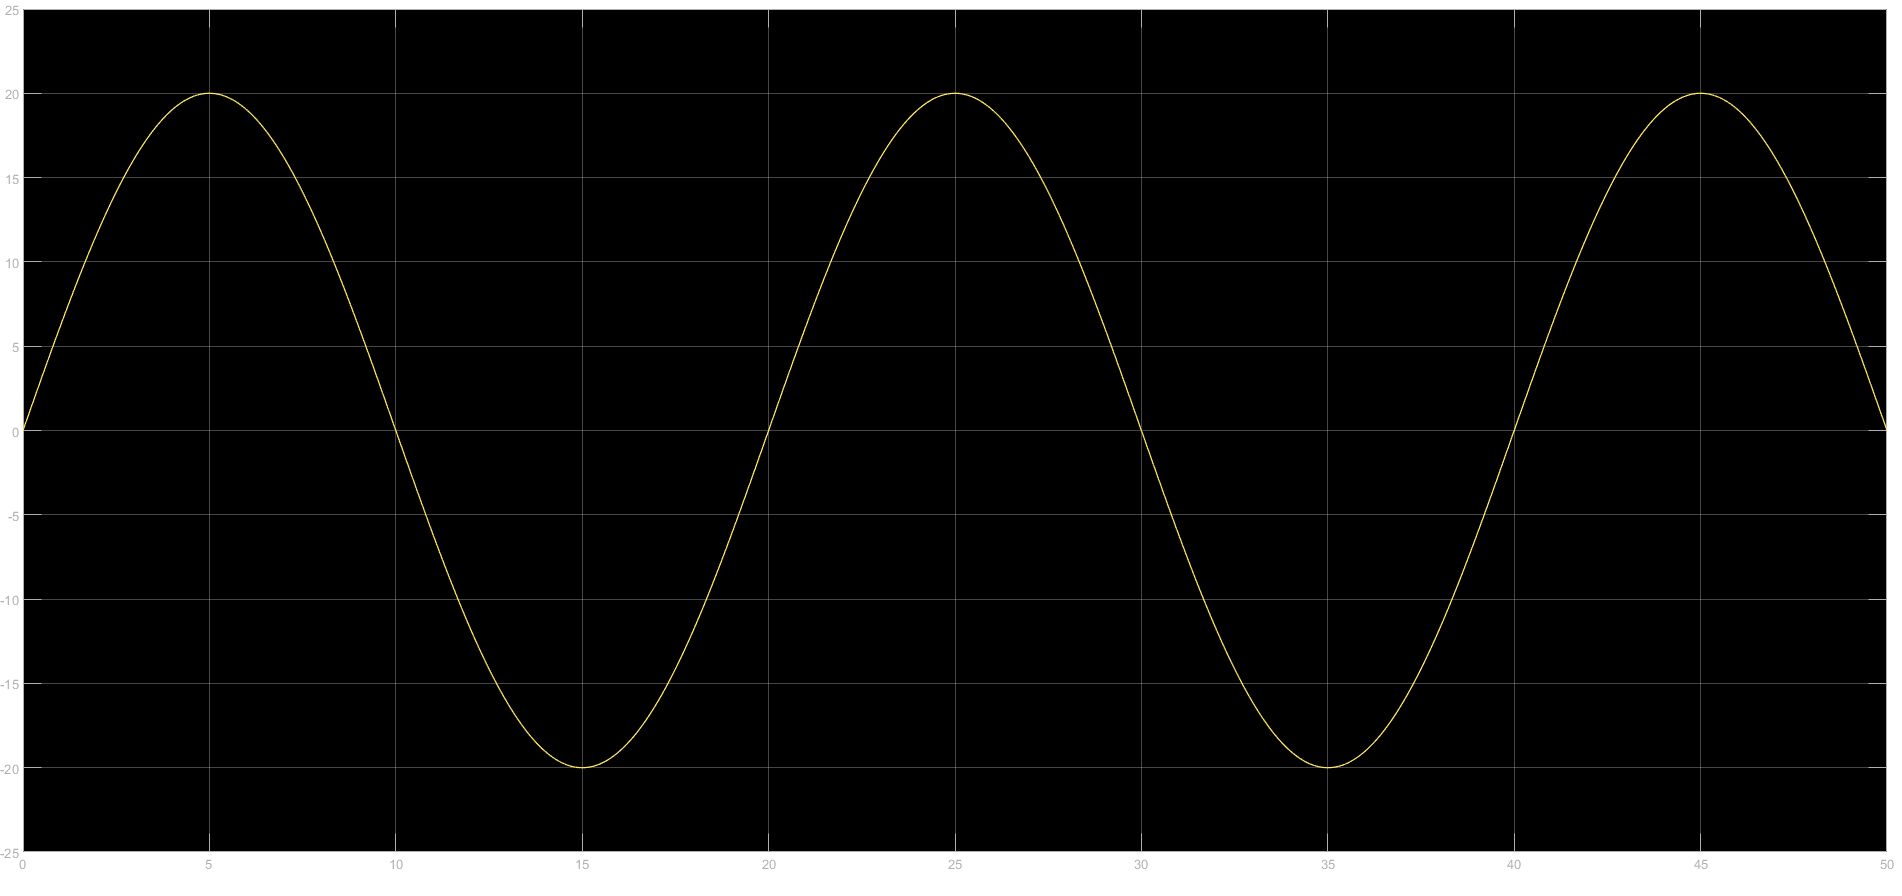
\includegraphics[width=\linewidth]{images/Sine_Reference.png}
    \caption{Sine Reference}
    \label{fig:reference}
\end{figure}

Figure \ref{fig:output:trajectory} shows the output trajectory y(t), figure \ref{fig:ControlInputHybrid} shows control input u(t), figure \ref{fig:Switch} shows the Mode Switch Signal S(t) and figure \ref{fig:Ref2Output} shows the reference alongside the output trajectory

\begin{figure}[htbp]
    \centering
    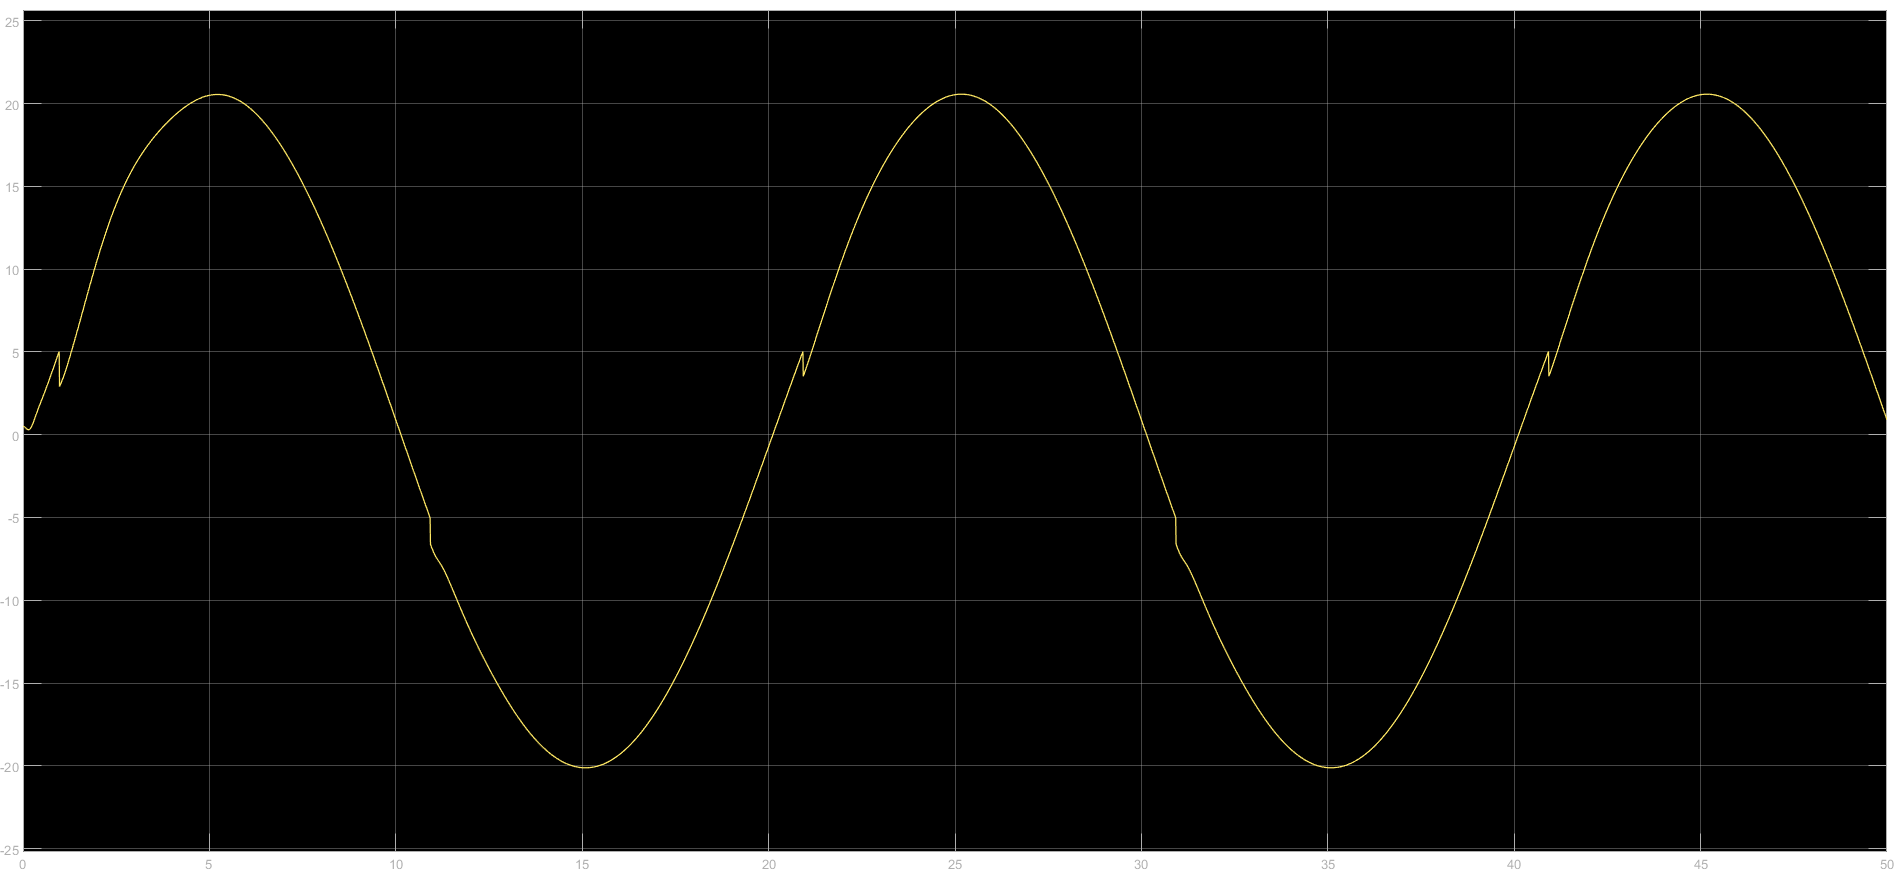
\includegraphics[width=\linewidth]{images/output_trajectory_hybrid.png}
    \caption{Output Trajectory}
    \label{fig:output:trajectory}
\end{figure}

\begin{figure}[htbp]
    \centering
    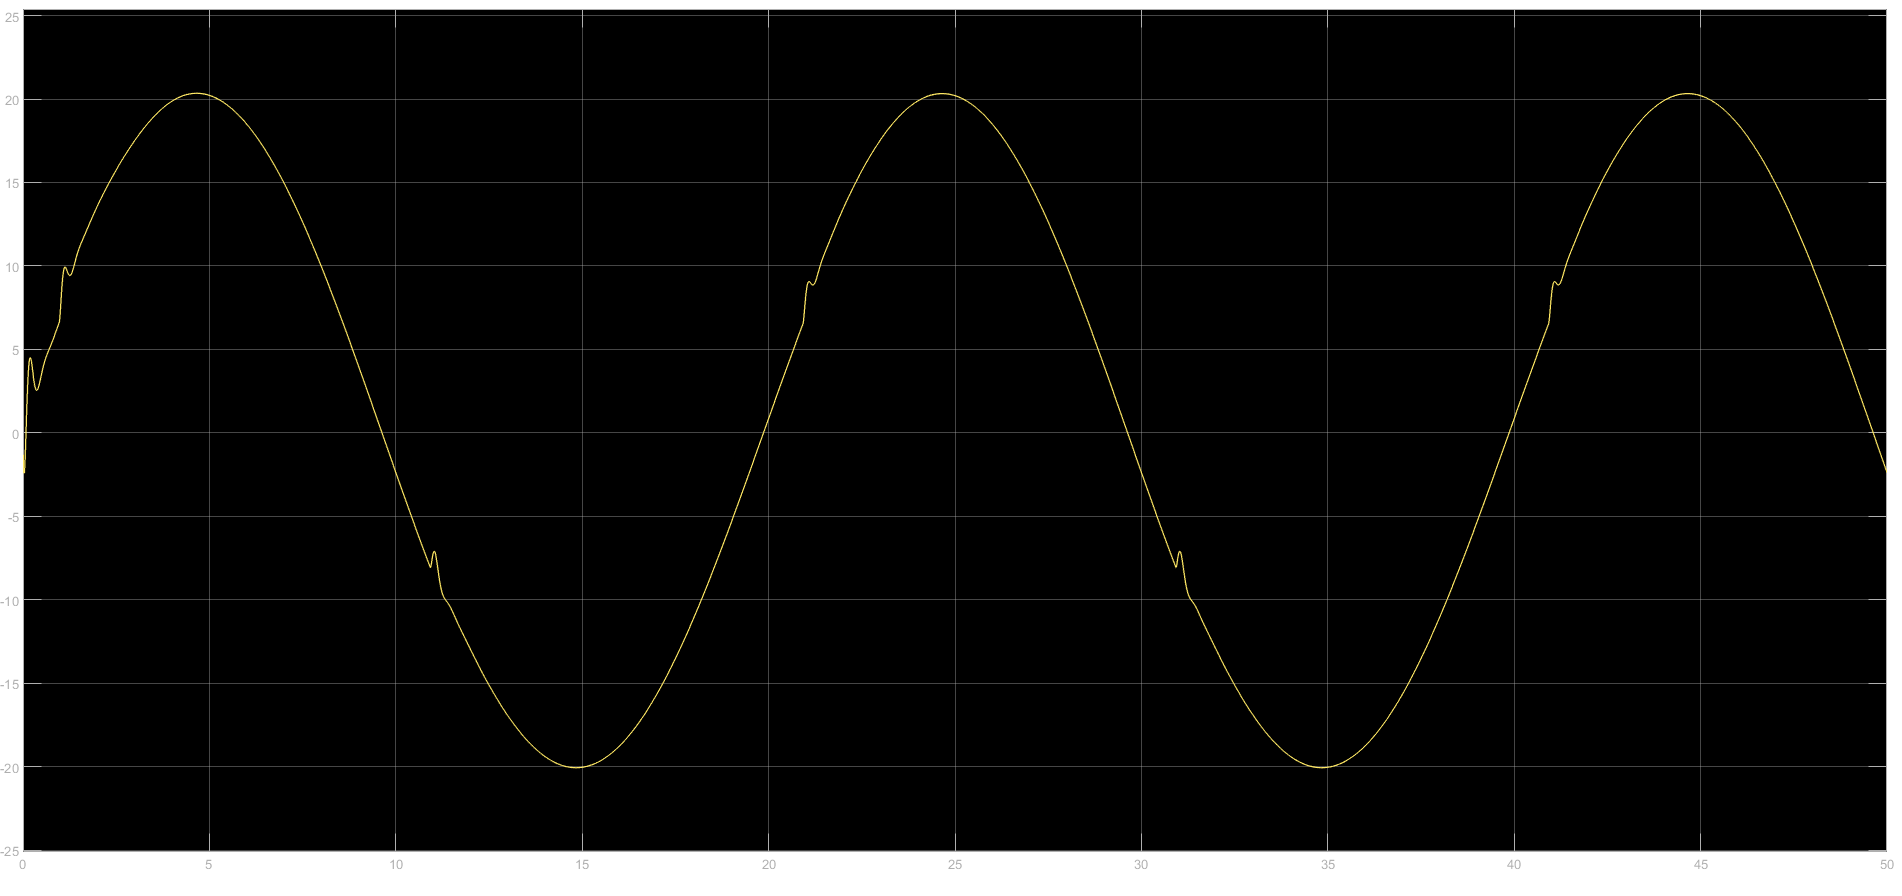
\includegraphics[width=\linewidth]{images/Control_Input_Hybrid.png}
    \caption{The Control Input in Hybrid}
    \label{fig:ControlInputHybrid}
\end{figure}

\begin{figure}[htbp]
    \centering
    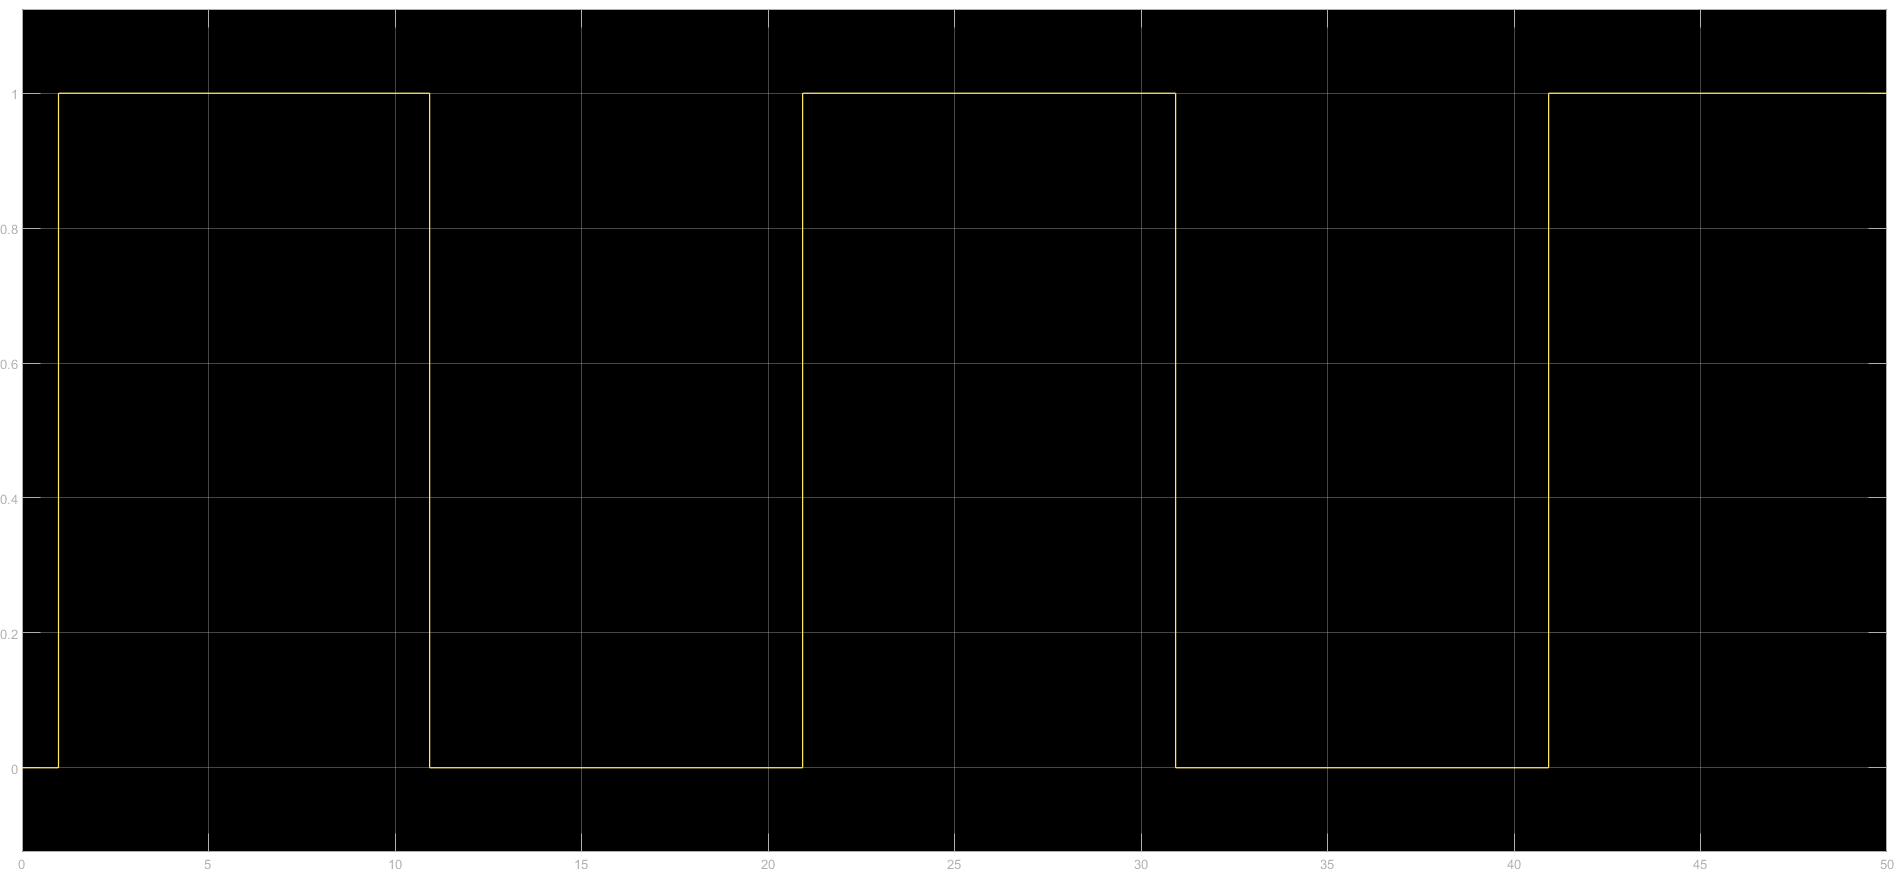
\includegraphics[width=\linewidth]{images/ModeSwitch.png}
    \caption{Mode Switch figure}
    \label{fig:Switch}
\end{figure}

\begin{figure}[htbp]
    \centering
    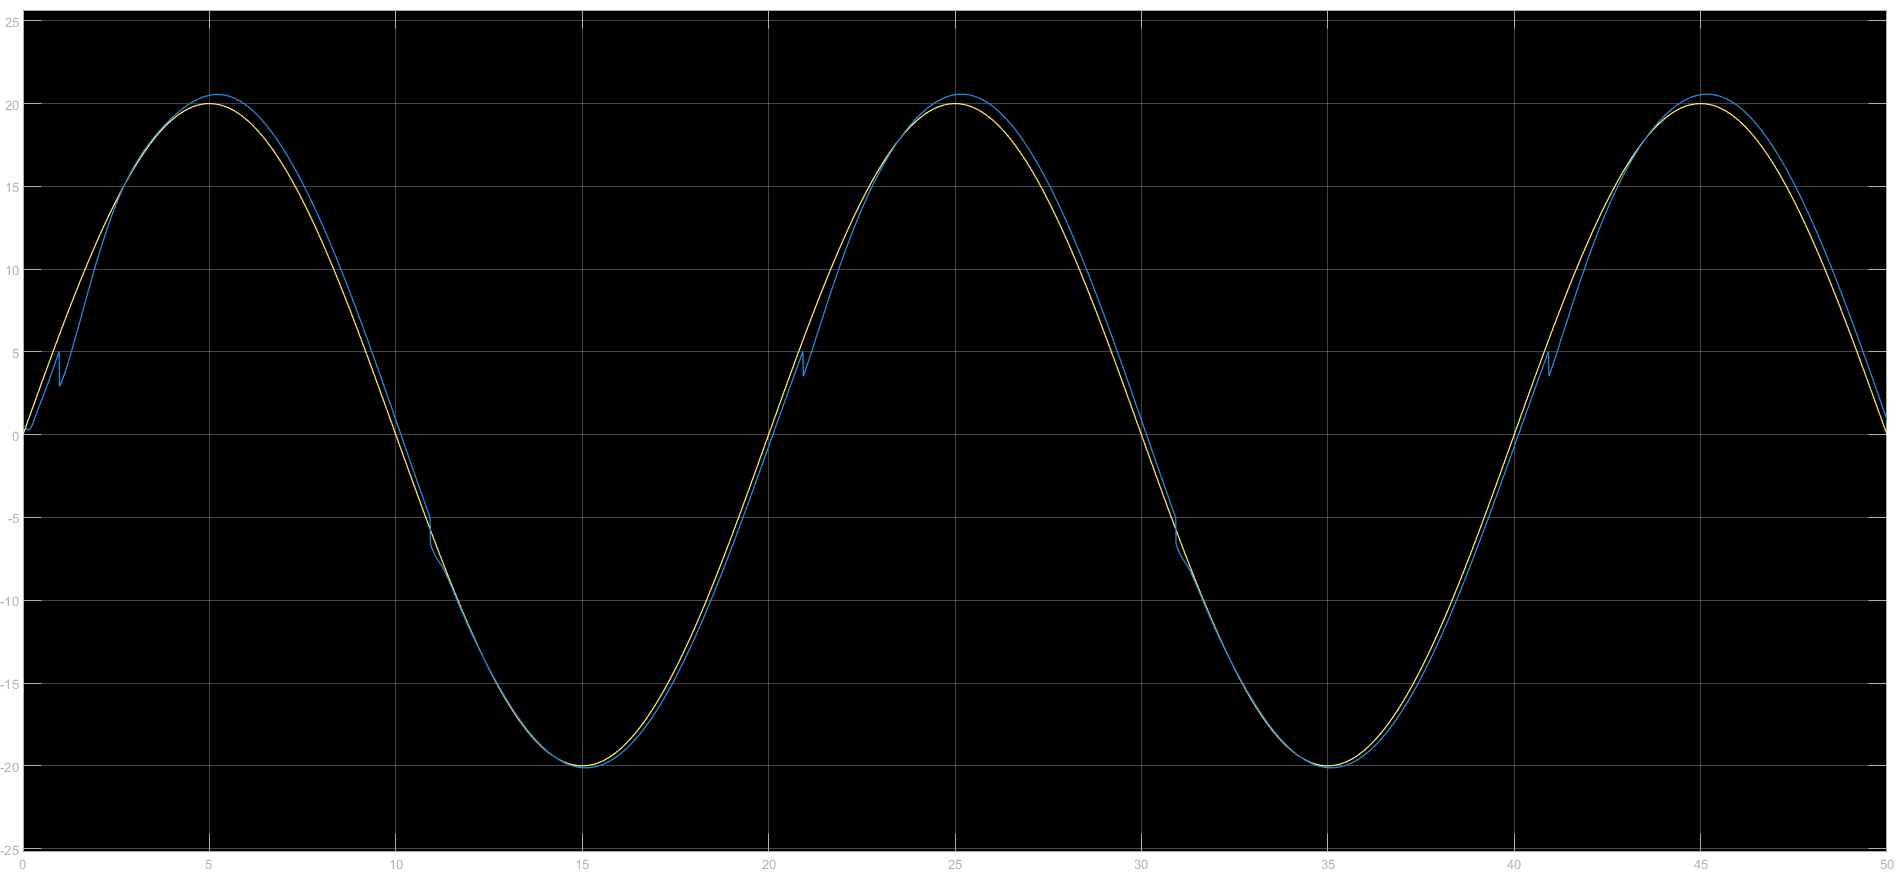
\includegraphics[width=\linewidth]{images/RefWithRespecttoOutput.png}
    \caption{Reference alongside Output with respect to time(t)}
    \label{fig:Ref2Output}
\end{figure}

The figures above show with switch changing dynamics roughly with a second delay the system experiences distortion in tracking the sinusoid system. It is also evident that there is a similarity between the Input signal and output signal, meaning that there is a distortion in the input signal as well. This mean that the MPC Controller, changes the the input signal based on the dynamic change it predicts in the future and can compensate for that in the output to obtain a more clear reference tracking in the output.

About the constraints that has been asked in the question, since the system was described in a way that did not reach the upper and lower bounds defined by the constraints, the output of the system does not differ for the "With Constraint" and the "Without Constraint" case.






\end{document}